% ****** Start of file apssamp.tex ******
%
%   This file is part of the APS files in the REVTeX 4.1 distribution.
%   Version 4.1r of REVTeX, August 2010
%
%   Copyright (c) 2009, 2010 The American Physical Society.
%
%   See the REVTeX 4 README file for restrictions and more information.
%
% TeX'ing this file requires that you have AMS-LaTeX 2.0 installed
% as well as the rest of the prerequisites for REVTeX 4.1
%
% See the REVTeX 4 README file
% It also requires running BibTeX. The commands are as follows:
%
%  1)  latex apssamp.tex
%  2)  bibtex apssamp
%  3)  latex apssamp.tex
%  4)  latex apssamp.tex
%
\documentclass[%
 reprint,
%superscriptaddress,
%groupedaddress,
%unsortedaddress,
%runinaddress,
%frontmatterverbose, 
%preprint,
%showpacs,preprintnumbers,
%nofootinbib,
%nobibnotes,
%bibnotes,
 amsmath,amssymb,
 aps,
%pra,
%prb,
%rmp,
%prstab,
%prstper,
%floatfix,
]{revtex4-1}

\usepackage{graphicx}% Include figure files
\usepackage{dcolumn}% Align table columns on decimal point
\usepackage{bm}% bold math
%\usepackage{hyperref}% add hypertext capabilities
%\usepackage[mathlines]{lineno}% Enable numbering of text and display math
%\linenumbers\relax % Commence numbering lines

%\usepackage[showframe,%Uncomment any one of the following lines to test 
%%scale=0.7, marginratio={1:1, 2:3}, ignoreall,% default settings
%%text={7in,10in},centering,
%%margin=1.5in,
%%total={6.5in,8.75in}, top=1.2in, left=0.9in, includefoot,
%%height=10in,a5paper,hmargin={3cm,0.8in},
%]{geometry}
\usepackage{pstricks,pst-node}
\usepackage[utf8]{inputenc}
\usepackage{float}
\usepackage[spanish]{babel}
\usepackage{amsmath}
\usepackage{hyperref}
\usepackage{tikz}
\usepackage{dsfont}
\usetikzlibrary{shapes.geometric, arrows}
\tikzstyle{startstop} = [rectangle, rounded corners, minimum width=3cm, minimum height=1cm,text centered, text width=2.5cm, draw=black, fill=magenta!10]
\tikzstyle{io} = [trapezium, trapezium left angle=70, trapezium right angle=110, minimum width=3cm, minimum height=1cm, text centered, text width=2.3cm, draw=black, fill=blue!10]
\tikzstyle{process} = [rectangle, minimum width=3cm, minimum height=1cm, text centered, text width=3cm, draw=black, fill=cyan!10]
\tikzstyle{decision} = [diamond, minimum width=3cm, minimum height=1cm, text centered, draw=black, text width=2.3cm,  fill=lime!20]
\tikzstyle{arrow} = [thick,->,>=stealth]

\begin{document}

\title{Longitud de onda de la luz}% Force line breaks with \\
\thanks{Usando la ley de difracción se calcula la longitud de onda y, posteriormente, se calcula la densidad de líneas en la rejilla de medición.}%

\author{Maria Sofía Álvarez López}%
\homepage{ms.alvarezl@uniandes.edu.co}
\affiliation{
 Universidad de los Andes\\
}%

\author{Sara María Varón Echeverri}
\homepage{sm.varon@uniandes.edu.co}
\affiliation{
Universidad de los Andes\\
}%

\date{\today}% It is always \today, today,
             %  but any date may be explicitly specified

\begin{abstract}
Los objetivos de éste laboratorio son dos: medir la longitud de onda emitida por un láser, usando el fenómeno de difracción, y, con la longitud de onda medida, determinar la densidad de líneas de una rejilla de difracción (con el fin de usar la rejilla más adelante en otros experimentos). Para el primer objetivo se midieron los valores promedio de diversas tomas de datos para la longitud de onda y se obtuvo un valor de $1694.09 \pm 735.54$ mm para los valores mínimos y de $1698.83 \pm 670.64$ mm para los máximos. Al comparar con el valor teórico 632.8 mm, el primer dato cuenta con un error porcentual del $167.6\%$ mientras que para el segundo fue de $168.4\%$. El error asociado a éstos resultados se haya en la exactitud más no en la precisión de la toma de datos y por tanto se plantean soluciones pertinentes al caso específico. Para la segunda parte, a partir de gráficas aproximadas, se muestra entonces la relación que existe entre la medida de las ranuras (d) y la medida de la ranura en sí (a) para varias ranuras, teniendo en cuenta que $d \approx \frac{1}{600}$ y $a \approx \frac{1}{3000}$. En esta parte, el error asociado a la medida de la longitud de onda fue mucho menor dados los instrumentos de medida y porque las distancias eran mucho mayores. El valor promedio obtenido fue de $\overline{\lambda} = 629,65  \pm 5 nm$, con tan sólo un error experimental del $\Epsilon = 0,49\%$.
\end{abstract}

\pacs{Valid PACS appear here}% PACS, the Physics and Astronomy
                             % Classification Scheme.
%\keywords{Suggested keywords}%Use showkeys class option if keyword
                              %display desired
\maketitle

%\tableofcontents

\section{\label{intro} Introducción y estado del arte}

Cuando la fuente de luz puntual es monocromática y es direccionada a un objeto opaco con bordes definidos, se espera que el resultado en la pantalla trasera sea una línea recta, simulando el borde definido del objeto. Sin embargo, esto no es así. Esta frontera no es nítida y se observa luz en la zona de la sombra y sombra en la zona de la luz. Esto es causado especialmente por la naturaleza ondulatoria de luz que genera interferencia consigo misma. 

\begin{figure}[H]
    \centering
    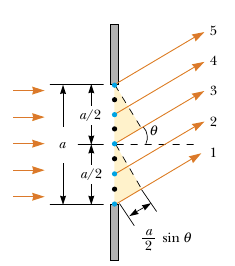
\includegraphics[scale= 0.6]{rayos}
    \caption{Al amplificar el montaje y tras el análisis pertinente del mismo, se encuentra que la luz no es un haz de luz sólida que se mueve y choca de forma geométrica con el objeto. Según el principio de Huygens, las diversas ondas secundarias chocan entre sí. De la mitad para arriba las ondas presentarán una naturaleza destructiva y de la mitad para abajo se presentará una naturaleza constructiva \cite{fisicauniversitaria}.}
    \label{fig:diagramaexplicativo}
\end{figure}

Es importante entender entonces el principio de Huygens para analizar éste fenómeno. $"$Este principio establece que cada punto de un frente de onda puede considerarse como una fuente de ondas secundarias, que se extienden en todas direcciones con rapidez igual a la de propagación de la onda$"$ \cite{fisicauniversitaria}. Por tanto, si se quisiera estudiar a cabalidad este fenómeno, se debería estudiar la amplitud y la fase relativa de cada una de éstas "ondas secundarias". Demás características del sistema deben ser definidas antes de proseguir con el estudio del resultado. Por ejemplo, la cercanía o lejanía de los objetos afecta el resultado. Si están cercanos debe utilizarse el método de difracción de Fresnel y, si están lejanos el uno del otro, se utiliza el método de difracción de Fraunhofer. Para encontrar los mínimos se utiliza la ecuación \eqref{(1)} y para encontrar los máximos se utiliza la ecuación \eqref{maximos}.

\begin{equation} \label{(1)}
    sen \theta = \frac{m\lambda}{a}
\end{equation}

\begin{equation} \label{maximos}
    a sen \theta = \frac{2n+1}{2} \lambda
\end{equation}

Ahora, es importante entender la diferencia entre una ranura y una rejilla de difracción. Por un lado, una ranura es sencillamente un espacio pequeño por el cual pasa el haz de luz. Por ejemplo, en la figura \ref{fig:diagramaexplicativo}, se muestra una ranura por la cuál pasa un haz de luz manteniendo la relación mostrada en la ecuación \eqref{(1)}. Por otro lado, una rendija de difracción es un material que cuenta con múltiples ranuras paralelas, todas del mismo tamaño y separadas por la misma distancia. Esto se muestra de manera gráfica en el diagrama \ref{fig:diagramarendija} que cumple con la ecuación \eqref{(2)}

\begin{figure}[H]
    \centering
    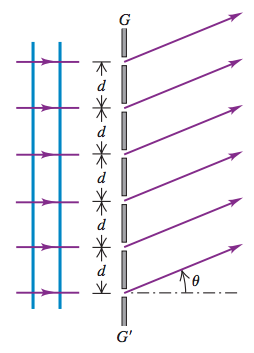
\includegraphics[scale= 0.5]{diagramarendija.png}
    \caption{Al amplificar el montaje de una rendija de difracción y tras el análisis pertinente del mismo, se halla una relación entre la distancia de las ranuras múltiples y el ángulo de incidencia de la luz en las mismas. Esta relación es explicada a cabalidad en la ecuación \ref{(2)} \cite{fisicauniversitaria}.}
    \label{fig:diagramarendija}
\end{figure}

\begin{equation} \label{(2)}
    d sen \theta = m\lambda
\end{equation}

En el caso de una rendija, como en la \ref{fig:diagramaexplicativo}, tenemos que:
\begin{figure}[H]
    \centering
    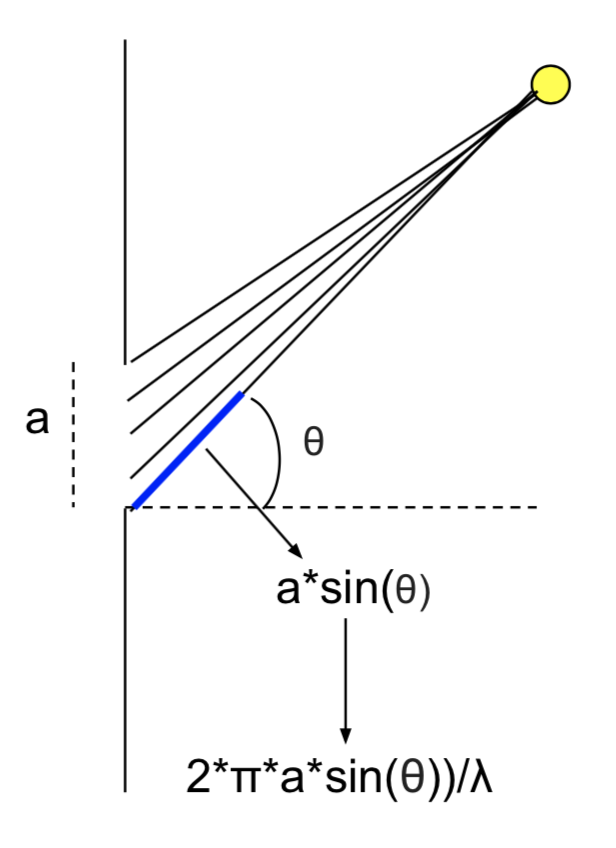
\includegraphics[scale= 0.5]{luz.png}
    \caption{Análisis téorico del experimento de la difracción con una rendija. A partir del diagrama, tomando un haz de luz, se pueden deducir las ecuaciones presentes en la imagen. (Elaboración personal).}
    \label{fig:figRayos}
\end{figure}
Con lo mostrado previamente, se puede determinar que:
\begin{equation}
    2\alpha = \frac{2\pi a \sin{\theta}}{\lambda}
\end{equation}
\begin{equation}
    A = 2R\sin{\alpha}
\end{equation}
Realizando un análisis más detallado de un único haz de luz, se tiene que:
\begin{figure}[H]
    \centering
    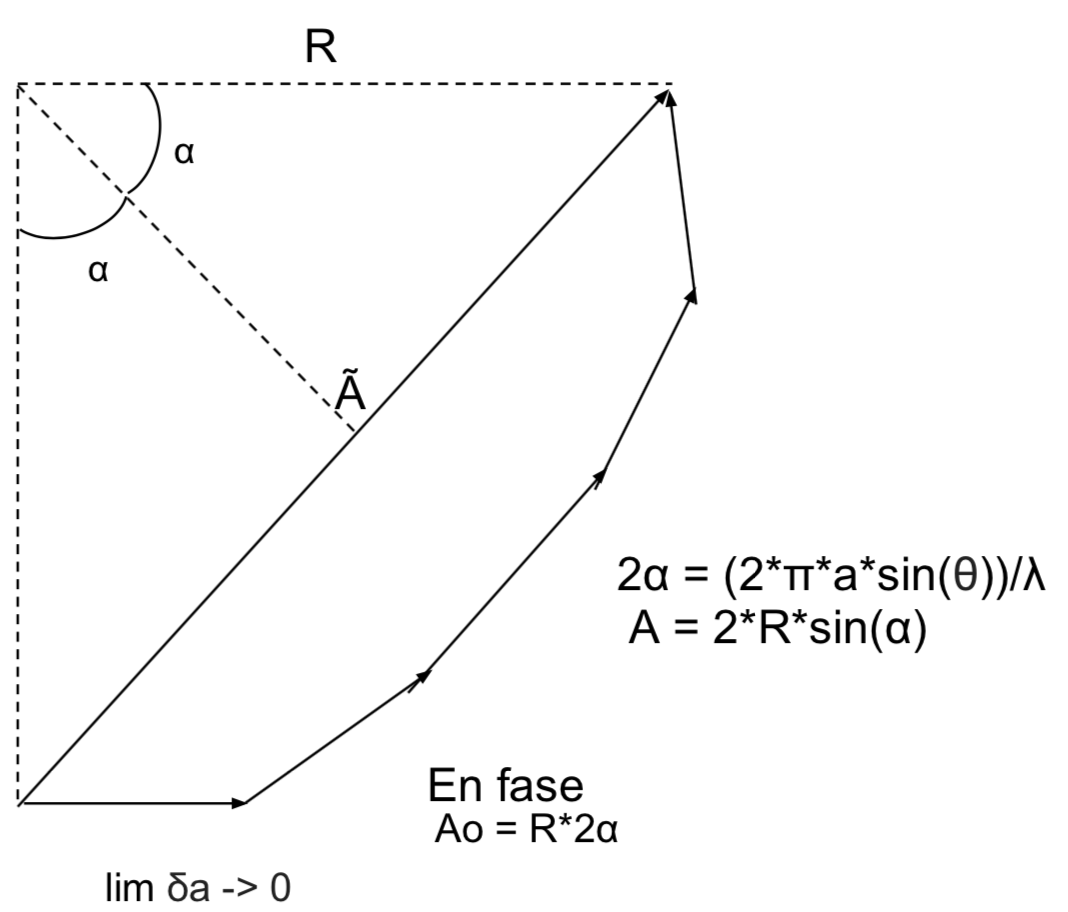
\includegraphics[scale= 0.4]{barco.png}
    \caption{Análisis téorico del experimento de la difracción con una rendija para un único haz de luz. Con trigonometría sencilla, pueden derivarse las ecuaciones presentes en la imagen. (Elaboración personal).}
    \label{fig:figBarco}
\end{figure}
Con todas las fórmulas obtenidas previamente, tenemos, entonces, que:
\begin{equation}
    A = A_{0}\frac{\sin{\alpha}}{\alpha}, \alpha = \frac{\pi a \sin{\theta}}{\lambda}
\end{equation}
Asimismo, tenemos que, para la intensidad que:
\begin{equation}
    I = I_{0}(\frac{\sin{\alpha}}{\alpha})^{2}
\end{equation}
Con lo anterior, entonces, tenemos que, para los mínimos:
\begin{equation}
    \alpha = n\pi
\end{equation}
\begin{equation}
  \frac{\pi a \sin{\theta}}{\lambda} = n\pi
\end{equation}
\begin{equation}
    a\sin{\theta}=n\lambda
\end{equation}

Por otro lado, para la rejilla de difracción, como la mostrada en la figura \ref{fig:diagramarendija}, es importante recalcar que la intensidad se calcula como:
\begin{equation}\label{intensidad}
    I = 4A_{0}[\frac{\sin{\alpha}}{\alpha}]^{2}[\sum_{p=1}^{N/2}\cos{(2p+1)\pi \frac{d}{\lambda}} \sin{\theta}]^2
\end{equation}
Cuando $N \longrightarrow \infty$, el término dominante de la expresión es el segundo, lo que permite calcular los máximos de la ecuación como:
\begin{equation}
    d\sin{\theta} = m \lambda, m \in \mathds{N}
\end{equation}

Finalmente, es lógico entonces pensar que el máximo de uno sea el mínimo del siguiente dada la naturaleza dual de la onda que atraviesa una de las ranuras. Si una onda es mitad constructiva y la otra mitad destructiva, para una sóla ranura se presenta un resultado específico. Para una red de de estas ranuras, el comportamiento individual se ve superpuesto con el de las demás ondas individuales. Por tanto, la frecuencia previamente expresada como constructiva es destruida por la de otra ranura y viceversa. 

\section{\label{montaje} Montaje experimental}

El experimento se dividió en dos partes principales con el fin de cumplir los dos objetivos específicos. En la primera parte, se utilizó un calibrador para generar ranuras angostas menores de 1 mm por las cuales se atravesó un láser de helio-neón. A una distancia previamente medida del calibrador se ubica una pantalla en la cuál se verá reflejado el patrón de difracción del láser. Dependiendo de la medida del ancho del calibrador (a) se presentarán diversos patrones para el mismo rayo. Luego, se miden las distancias del centro del espectro a cada una de las líneas longitud de onda, tanto para los mínimos como para los máximos. Medir la distancia entre mínimos es mejor que medir la distancia entre máximos dado que la delimitación entre ellas es mucho más clara y ya que se mantiene consistencia entre medidas.

\begin{figure}[H]
    \centering
    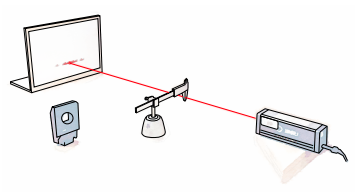
\includegraphics[scale= 0.5]{Montaje.png}
    \caption{El diagrama anterior muestra claramente el montaje experimental a armar y los elementos o materiales que serán utilizados. Para el desarrollo del experimento se utilizará un láser, un calibrador, una rejilla de difracción, una regla, y un cuaderno o un libro de papel delgado.}
    \label{fig:montaje}
\end{figure}

Posteriormente, para la segunda parte del experimento, se utiliza el mismo rayo de helio-neón por una rejilla de difracción. Se miden los ángulos que salen de los rayos difractados utilizando la medida de la distancia de la rejilla conforme a la pantalla. Con estos datos obtenidos será posible entonces medir la intensidad de líneas como se muestra en la ecuación \eqref{intensidad}.

\section{\label{resultados} Resultados y análisis}

Dada la primera parte del experimento, utilizando la ley de difracción para una rendija, se midió la longitud de onda de la luz del láser. Mediante la medición de la distancia entre mínimos y máximos conforme el centro y conforme a la regresión lineal planteada en las ecuaciones \eqref{(1)} y \eqref{maximos}, se encontraron diversas aproximaciones al valor esperado. Los datos tomados se muestran en la tabla \ref{fig: datos}.

\begin{figure}[H]
    \centering
    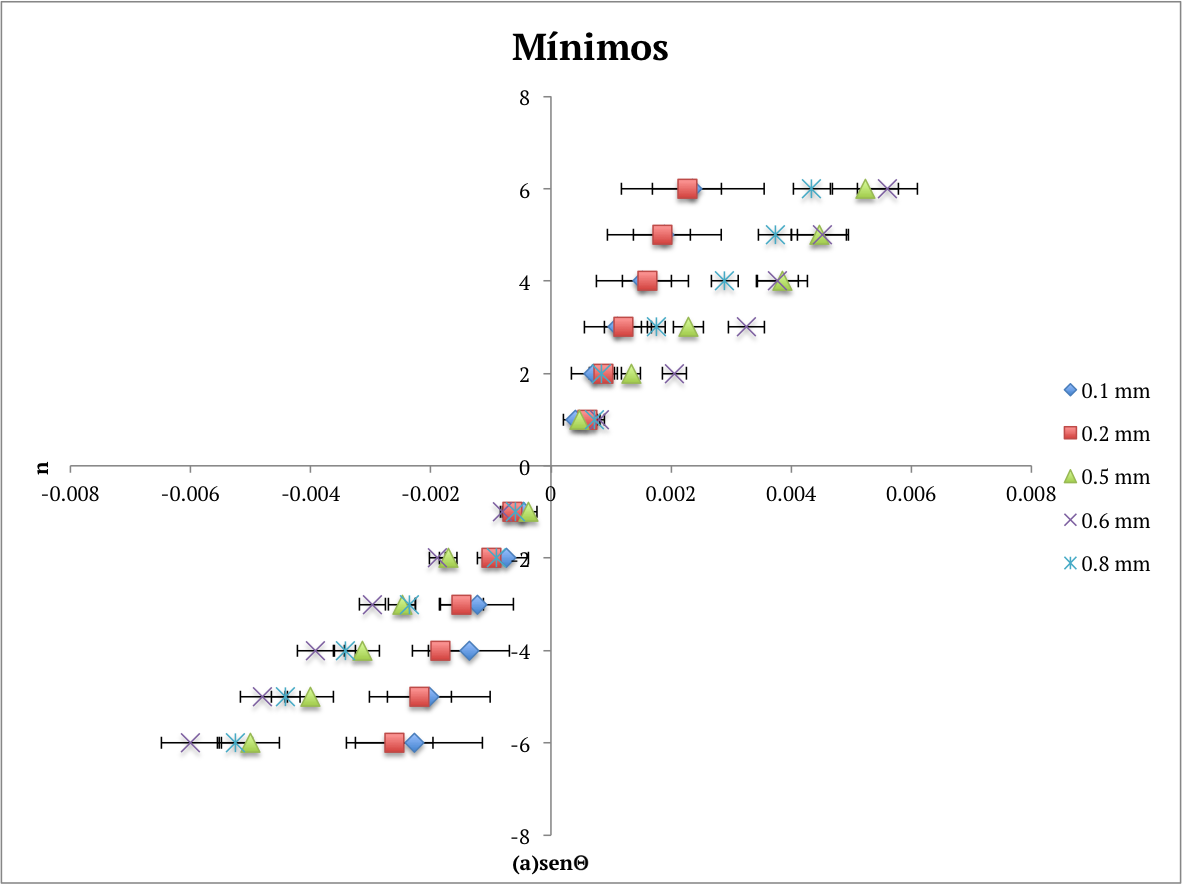
\includegraphics[scale= 0.43]{minimos.png}
    \caption{Dadas las cinco diferentes medidas de la amplitud de la rendija, se graf'ica dada la ecuación \eqref{(1)}. Por tanto, la medida de la pendiente es igual a la longitud de onda de la luz del láser. Dado que n no tiene unidades y no hace referencia a un medida específica, no hay barras de error correspondientes a éste valor.}
    \label{fig:minimos}
\end{figure}

\begin{figure}[H]
    \centering
    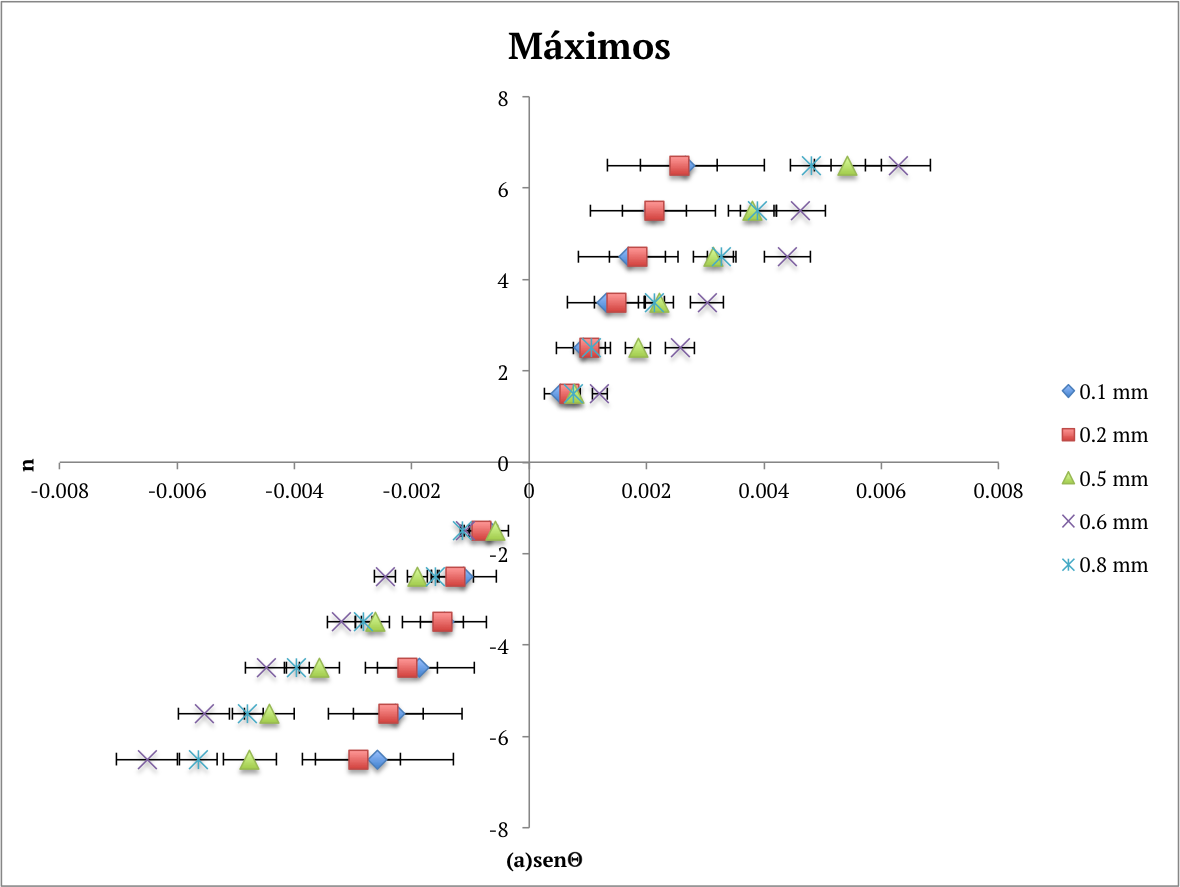
\includegraphics[scale= 0.43]{maximos.png}
    \caption{Dadas las cinco diferentes medidas de la amplitud de la rendija, se graf'ica dada la ecuación \eqref{maximos}. Por tanto, la medida de la pendiente es igual a la longitud de onda de la luz del láser. Dado que n no tiene unidades y no hace referencia a un medida específica, no hay barras de error correspondientes a éste valor.}
    \label{fig:maximos}
\end{figure}

\begin{table}[H]
  \centering
  \caption{Información del resultado del análisis de las gráficas. La pendiente, teniendo en cuenta las ecuaciones \eqref{(1)} y \eqref{maximos}, la pendiente debe ser igual la longitud de onda de luz que sale del láser, en este caso, de 632.8 mm. El promedio para los valores del lambda calculados con los mínimos es de $1694.09 \pm 735.54$ mm, mientras que el promedio con los valores máximos es de $1698.83 \pm 670.64$ mm.}
    \begin{tabular}{|r|l|r|r|}
    \hline
    \multicolumn{1}{|l|}{a} & Pendiente & \multicolumn{1}{|l|}{Punto de} & \multicolumn{1}{|l|}{Coeficiente de} \\
    \multicolumn{1}{|l|}{$\pm 0.05 mm$} & [mm]  & \multicolumn{1}{|l|}{corte [mm]} & \multicolumn{1}{|l|}{ correlación} \\
    \hline
    \multicolumn{4}{|c|}{Mínimo} \\
    \hline
    0.10  & $2606.75 \pm 0.43$ & 0.0166 & 0.99763 \\
    0.20  & $2371.95 \pm 1.06$ & 0.271 & 0.99415 \\
    0.50  & $1180.99 \pm 1.68$ & 0.0937 & 0.99308 \\
    0.60  & $1037.16 \pm 0.41$ & 0.0321 & 0.99772 \\
    0.80  & $1273.61 \pm 2.64$ & 0.2846 & 0.9855 \\
    \hline
    \multicolumn{4}{|c|}{Máximo} \\
    \hline
    0.10  & $2496.09 \pm 0.19$ & 0.1381 & 0.99658 \\
    0.20  & $2347.20 \pm 0.52$ & 0.2129 & 0.99193 \\
    0.50  & $1322.48 \pm 2.08$ & 0.0635 & 0.99414 \\
    0.60  & $1042.26 \pm 0.91$ & 0.0911 & 0.99586 \\
    0.80  & $1286.14 \pm 1.90$ & 0.3899 & 0.99633 \\
    \hline
    \end{tabular}%
  \label{tab:longitud de onda}%
\end{table}%

El promedio de los datos para la medida de la longitud de onda obtenida de las medidas de los mínimos es igual a $1694.09 \pm 735.54$ mm, mientras que el promedio para la medida de los máximos es igual a $1698.83 \pm 670.64$ mm. Teniendo en cuenta que el valor esperado era de 632.8 mm, se puede decir que ambas medidas están desfasadas por más de 1000 mm, aproximadamente. Al analizar los datos de la tabla \ref{tab:longitud de onda}, se encuentra que todos los datos tienen éste tipo de error pero no varían de manera significante entre sí, dadas las desviaciones estándar de las medidas. De esto se deduce que el experimento no tuvo errores de precisión pero sí de exactitud. Las medidas fueron afectadas por alguna fuente error sistemática que afectó el desarrollo del experimento como un todo, sin desviar aleatoriamente los valores. \\
Para la segunda parte del laboratorio, se tomó una rejilla de difracción (o rendija múltiple) con la cual se varió la distancia L y se midieron las distancias entre los patrones de orden 1 y 2 al patrón de orden 0. Con esto, utilizando la ecuación (12), sería posible calcular la longitud de onda $\lambda$ correspondiente a cada distancia \textit{L} entre la pantalla y la rejilla. Lo anterior se muestra con mayor claridad en el diagrama a continuación: 

\begin{figure}[H]
    \centering
    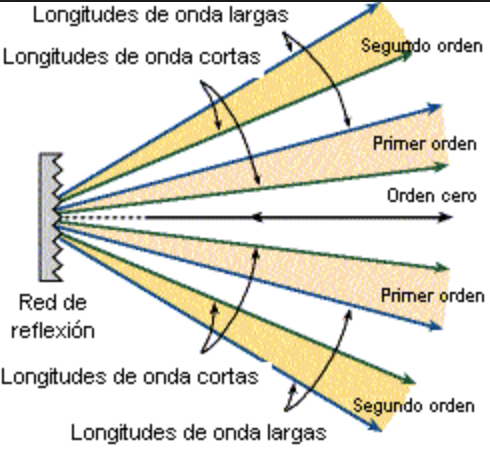
\includegraphics[scale= 0.5]{laseradventure.png}
    \caption{Como se observa en la imagen, al traspasar un haz de luz por una rejilla de difracción, se generan patrones de varios órdenes. El orden 0 no sufre ningún fenómeno de difracción, mientras que los de orden 1 y orden 2 sí sufren fenómenos de difracción a ciertos ángulos específicos, según la distancia \textit{L} a la que se encuentra la rejilla de la pantalla.}
    \label{fig:maximos}
\end{figure}

A partir de lo anterior, para los puntos generados por cada orden, obtuvimos los siguientes datos. En las tablas a continuación se presentan los valores de \textit{L [mm]},y las distancias, \textit{d [mm]}, entre los puntos de los ordenes determinados para dichas longitudes. Con lo anterior, fue posible calcular $\arctan(\frac{d}{L})$ (como el ángulo $\theta$ al que el haz se difracta respecto a la rejilla), $\sin{(\arctan(\frac{d}{L}))}$ y la longitud de onda correspondiente a cada ensayo efectuado. 

\begin{table}[H]
\begin{tabular}{|c|c|c|c|c|} \hline
\label{tabla1s}
L ($mm \pm 0.5$) & d ($mm \pm 0.5$)    & $\arctan(d/L)$      & $\sin{\theta}$        & $\lambda \pm 5 nm$      \\ \hline
45     & 21   & 0,43662  & 0,42289 & 704,81 \\ \hline
105    & 43   & 0,38868 & 0,378976 & 631,63 \\ \hline
80     & 35   & 0,41241 & 0,400819 & 668,03   \\ \hline
60     & 27   & 0,42285 & 0,410365 & 683,94 \\ \hline
50     & 23,5 & 0,43936 & 0,425361  & 708,94 \\ \hline
\end{tabular}  
\caption{En este cuadro, se muestran los valores obtenidos para la longitud de onda de la luz, en el experimento de la difracción con una rejilla, para los máximos de difracción de orden 1. Como se observa en la tabla, se obtuvieron resultados bastante precisos (cercanos entre sí) y exactos, respecto al valor experimental de $\lambda = 632,8 nm$. Cabe aclarar que $\arctan(d/L) = \theta$}
\end{table}

A partir de los datos de la tabla, obtuvimos una longitud de onda promedio $\overline{\lambda} = 679,47 nm \pm 5$, con tan sólo un error experimental del $\epsilon = 7,37\%$. Esto sustenta el hecho de que esta parte del experimento tiene una exactitud experimental mucho más elevada que la primera, puesto que, en este, era mucho más sencillo tomar las medidas entre los máximos de cada orden.   

Para los máximos de orden 2, obtuvimos los siguientes datos:
\begin{table}[H]
\begin{tabular}{|c|c|c|c|c|}
\label{tabla2s}
\hline
L ($mm \pm 0.5$) & d ($mm \pm 0.5$)    & $\arctan(d/L)$      & $\sin{\theta}$        & $\lambda \pm 5 nm$      \\ \hline
45  & 51      & 0,84782 & 0,74984 & 624,86 \\ \hline
105 & 119     & 0,84782 & 0,74984 & 624,86 \\ \hline
80  & 94      & 0,86568 & 0,76154  & 634,62 \\ \hline
60  & 74      & 0,88950 & 0,77676 & 647,30 \\ \hline
50  & 55      & 0,83298 & 0,73994 & 616,62 \\ \hline
\end{tabular} \caption{En este cuadro, se muestran los valores obtenidos para la longitud de onda de la luz, en el experimento de la difracción con una rejilla, para los máximos de difracción de orden 2. Como se observa en la tabla, se obtuvieron resultados bastante precisos (cercanos entre sí) y exactos, respecto al valor experimental de $\lambda = 632,8 nm$. Cabe aclarar que $\arctan(d/L) = \theta$.}
\end{table}

A partir de los datos de la tabla, obtuvimos una longitud de onda promedio $\overline{\lambda} = 629,65  \pm 5 nm$, con tan sólo un error experimental del $\epsilon = 0,49\%$. Esto sustenta el hecho de que esta parte del experimento tiene una exactitud experimental mucho más elevada que la primera, puesto que, en este, era mucho más sencillo tomar las medidas entre los máximos de cada orden. 

Después de haber analizado el comportamiento de la intensidad del haz respecto al ángulo $\theta$ al que cada uno se difracta, se decidió que resultaba conveniente analizar los resultados de la intensidad respecto al $\sin{(\theta)}$. Los resultados obtenidos se presentan a continuación. \\    
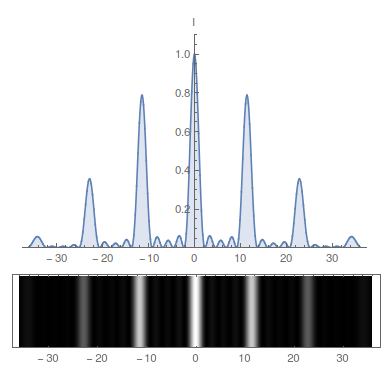
\includegraphics[scale= 0.5]{5.png}

Figura 9.1 Gráfica de la intensidad (I) contra el $\sin{(\theta)}$ para una rejilla con $n=5$ rendijas. El estudio detallado de las gráficas se realizará más adelante. \\

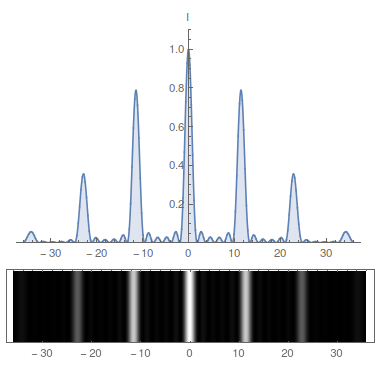
\includegraphics[scale= 0.5]{6.png}

Figura 9.2 Gráfica de la intensidad (I) contra el $\sin{(\theta)}$ para una rejilla con $n=6$ rendijas. El eestudio detallado de cada gráfica se realizará más adelante. \\

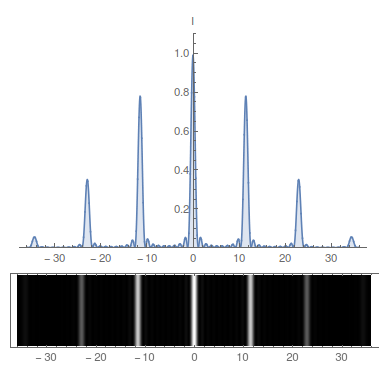
\includegraphics[scale= 0.5]{10.png}

Figura 9.3 Gráfica de la intensidad (I) contra el $\sin{(\theta)}$ para una rejilla con $n=6$ rendijas. El eestudio detallado de cada gráfica se realizará más adelante. \\

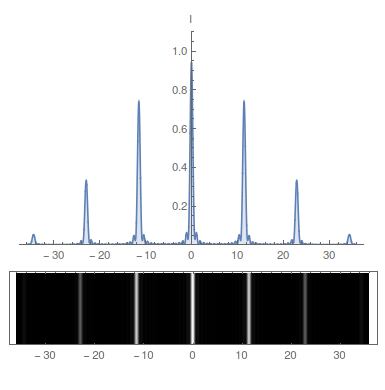
\includegraphics[scale= 0.5]{15.png}

Figura 9.4 Gráfica de la intensidad (I) contra el $\sin{(\theta)}$ para una rejilla con $n=6$ rendijas. El eestudio detallado de cada gráfica se realizará más adelante. \\

Como se observa en las imágenes, para un número pequeño de rendijas (Ver gráficas 9.1 y 9.2 con $n=5,6$, respectivamente) los mínimos, correspondientes a la anchura de la rendija (\textit{a}), se pueden contemplar a simple vista en la gráfica. No obstante, en el patrón de interferencia, estos son casi invisibles, puesto que la intensidad presentada por los máximos (asociados al espaciado entre rendijas (\textit{d}) es mucho mayor. En el caso de las figuras 9.3 y 9.4, estos mínimos son aún mucho más pequeños, pues el ancho de los máximos asociados a d es mucho menor, haciendo que, en estos casos, sean casi imposibles de contemplar. Lo anterior ocurre puesto que $a \approx \frac{d}{5}$, haciendo que $a \ll d$. En todos los casos, el pico de la función se centra en 0, donde no ocurre ningún fenómeno de difracción ('máximo' de orden 0). Desde allí empiezan a aparecer los siguientes órdenes de máximos hacia ambos lados del pico máximo. Aunque en las gráficas es posible contemplar los máximos hasta de tercer orden, en el experimento sólo se pudieron ver los máximos de primer y segundo orden. Para poder alcanzar a visualizar más máximos, sería necesario tener un montaje experimental más preciso y sofisticado. \\

A partir de las gráficas anteriores, se muestra entonces la relación que existe entre la medida de las ranuras (d) y la medida de la ranura en sí (a) para varias ranuras. En todas estas gráficas es posible visualizar que la intensidad disminuye conforme aumenta, en valor absoluto, el seno del ángulo de difracción. Conforme se ve en las gráficas, la amplitud entre éstas "campanas" de valores máximos es proporcional a la medida de d mientras que la distancia entre crestas para los mínimos son proporcionales a a, teniendo en cuenta que $d \approx \frac{1}{600}$ y $a \approx \frac{1}{3000}$. El pico máximo de la función, en todos los casos, se centra en 0, pues, en el orden 0 no ha ocurrido ningún fenómeno de difracción. Esto implica que estos valores son los que tienen una mayor intensidad, como se ve en la pantalla mostrada en cada una de las imágenes. Conforme aumenta el orden de los máximos, la intensidad de la luz asociada a ellos disminuye. Lo anterior, puesto que el ángulo de difracción es mayor. Estas crestas corresponden a los máximos para una rejilla de difracción. Los mínimos, por su parte, corresponden a la intensidad de \textit{a}. Claramente, debido a que $a \ll d$, estos valores serán muchísimo menores que los de los máximos, presentando una intensidad muchísimo menor que la de los máximos asociados a \textit{d}. Incluso, para algunos valores de N ($N = 10,15$) (cantidad de rendijas), es casi que despreciable.  


\section{\label{conclusiones} Conclusiones}

En conclusión, se logró medir la longitud de onda emitida por un láser, usando el fenómeno de difracción. A pesar de que los resultados fueron congruentes con la teoría y en todas las gráficas mostradas se puede hacer un ajuste lineal bueno con valores entre 0.98 y 0.99 (ver valores del coeficiente de correlación en la tabla \ref{tab:longitud de onda}), el resultado para la medida de la longitud de onda de la luz no fue el esperado. Por un lado, para los valores mínimos se obtuvo un promedio de $1694.09 \pm 735.54$ mm, mientras que el promedio con los valores máximos fue de $1698.83 \pm 670.64$ mm. Al comparar con el valor teórico 632.8 mm, el primer dato cuenta con un error porcentual del $167.6\%$ mientras que para el segundo fue de $168.4\%$. Estos errores se explican dada la naturaleza del laboratorio y los instrumentos de medida utilizados. Todas las medidas fueron hechas con un calibre de incertidumbre asociada 0.05 mm para medidas que luego serían expuestos a muchos tratamientos y medidas distintas. Adicionalmente, las longitudes de onda medidas no eran fácilmente visibles y, por tanto, se genera un error sistemático en la toma de medidas, afectando la exactitud pero no la precisión. Prueba de esto es que todas las medidas están distanciadas 1000 mm del valor esperado, entonces, se puede decir que el valor asociado se mantiene constante en la toma de datos.

Con el fin de disminuir las fuentes de error de éste experimento, se plantea la opción de usar redes de difracción de Bragg, ya que estas generan un rayo de una sóla longitud de onda y utilizan fibras ópticas para mejorar la precisión de las medidas \cite{Bragg}. Adicionalmente, se plantea la opción de utilizar algún tipo de ampliador para que se vean de manera más clara las longitudes de onda o, en su defecto que se utilicen otro tipo de métodos para el estudio de las ondas electromagnéticas. Por ejemplo, al utilizar un difractómetro de rayos X, un espectro de fluorescencia de rayos X y demás instrumentos se generan mayores valores para las longitudes de onda y consecuentemente que los instrumentos de medida no presenten una incertidumbre tan grande comparada con los datos obtenidos \cite{rayos_x}. Éste método, conocido generalmente como el "powder diffraction" o difracción de rayos X ha demostrado tener diversas ventajas en la investigación sobre modelos físicos y, por tanto, no se muestra relevante para la investigación presente \cite{powder_diffraction}. Demás maneras para procurar la exactitud de este experimento podrán ser tomadas en futuros laboratorios.

Para la segunda parte, con la longitud de onda medida, se logró determinar la densidad de líneas de una rejilla de difracción. Teniendo en cuenta que los instrumentos de medida sí tenían una incertidumbre que fuera coherente con las medidas tomadas ya que éstas fueron de mucha más magnitud, se obtuvo un dato promedio de $\overline{\lambda} = 629,65  \pm 5 nm$, con un error experimental del $\Epsilon = 0,49\%$ conforme al dato teórico. Demostrado así, la disminución de las fuentes de error en los instrumentos de medida se muestran determinantes para el análisis posterior de los resultados. Adicionalmente, se estudia con éxtio la longitud de onda presentada. Por otro lado, a partir de las gráficas mostradas de la intensidad de las líneas versus $seno(\theta)$, se explica entonces la relación que existe entre la medida de las ranuras (d) con la amplitud entre éstas "campanas" de valores máximos y la medida de la ranura en sí (a) conforme a la distancia entre crestas para los mínimos para diferentes cantidades de ranuras. Para este experimento, teniendo en cuenta que $d \approx \frac{1}{600}$ y $a \approx \frac{1}{3000}$, las graficas mostradas son las esperadas y se estudia correspondientemente que la densidad de líneas de difracción sí se comportan de la manera esperada.

\bibliography{biblio}

\end{document}